%%%%%%%%%%%%%%%
%APPENDIX A
%%%%%%%%%%%%%%%

\chapter{\label{appendixA}Simulation and Spirometry Data}
\markboth{Appendix A - Simulation and Spirometry Data}{}

This section presents the measures obtained from spirometry and simulation on three subjects. Each subject was asked to breathe in a steady fashion in three different positions: standing, sitting and lying. For each position, they had to breathe normally (quiet breathing) and then more energetically (forced breathing) by making large breaths. 
\\
\\
The resulting data was first processed to make any comparison possible as explained in chapter \ref{ch:validation}, section \ref{sec:prep_data}.

\newpage
\section{\label{appendixA:p1}Subject 1}

\begin{figure}[H]
	\centering
	 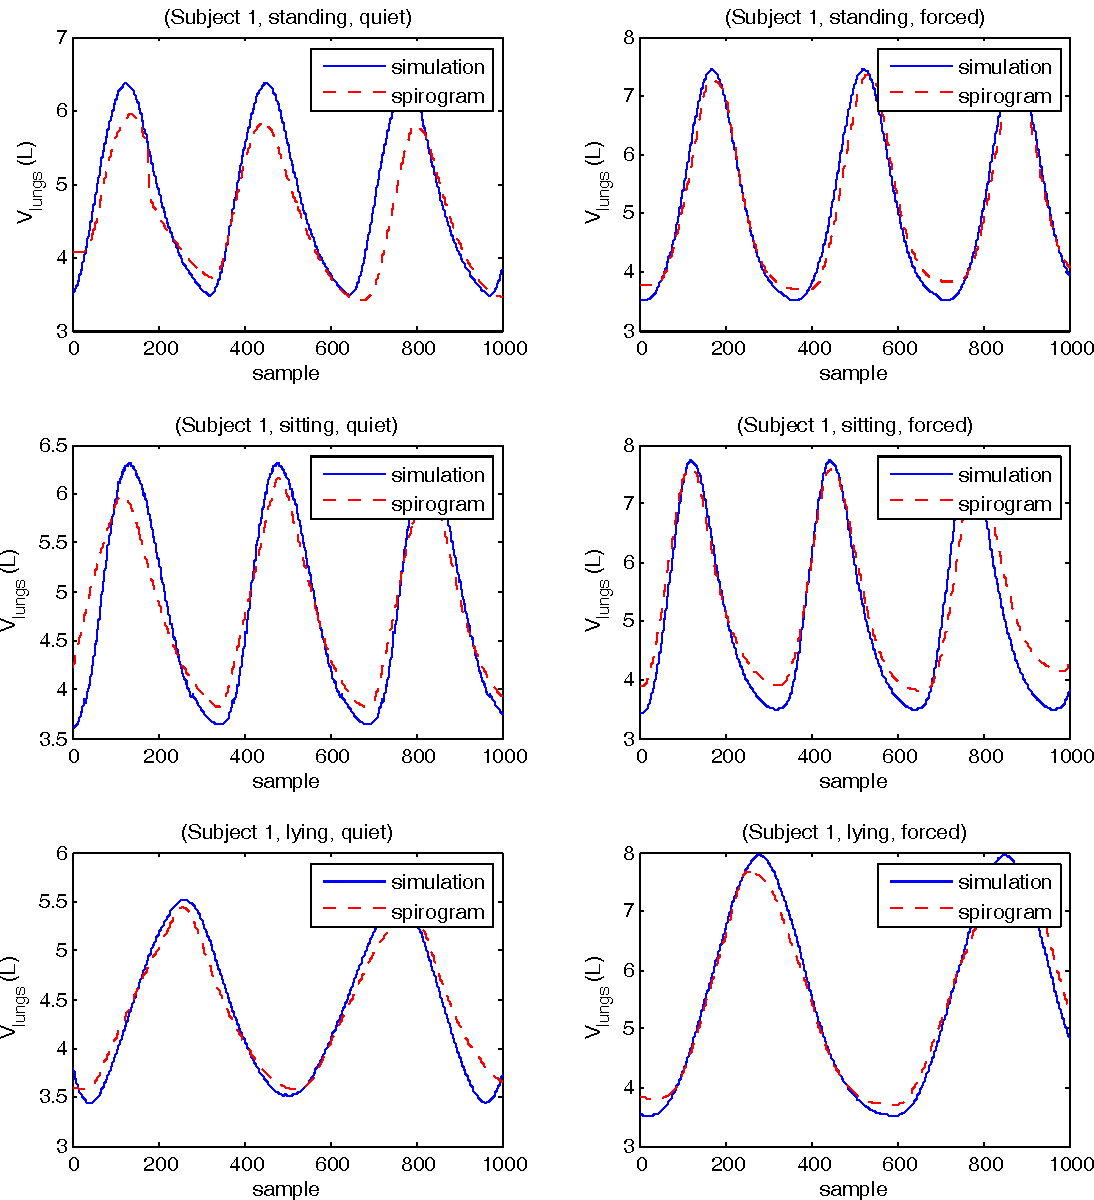
\includegraphics[width=1\textwidth]{pics/th}
	\caption[Simulation and spirometry data from subject 1]{\label{appA:fig:p1}Simulation and spirometry data from subject 1.}
\end{figure}

\newpage
\section{\label{appendixA:p2}Subject 2}

\begin{figure}[H]
	\centering
	 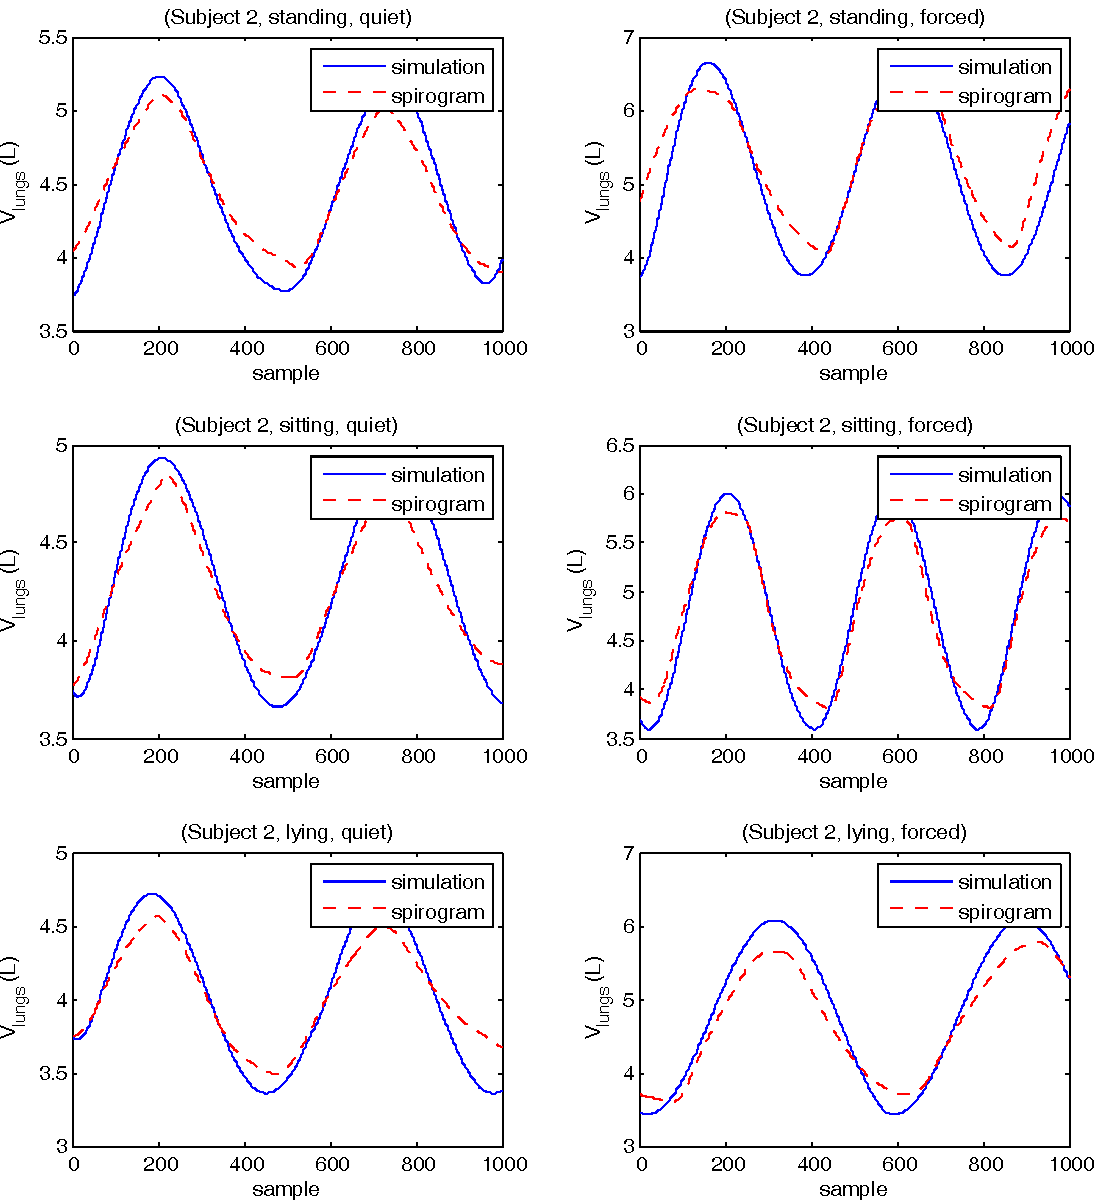
\includegraphics[width=1\textwidth]{pics/j}
	\caption[Simulation and spirometry data from subject 2]{\label{appA:fig:p2}Simulation and spirometry data from subject 2.}
\end{figure}

\newpage
\section{\label{appendixA:p3}Subject 3}

\begin{figure}[H]
	\centering
	 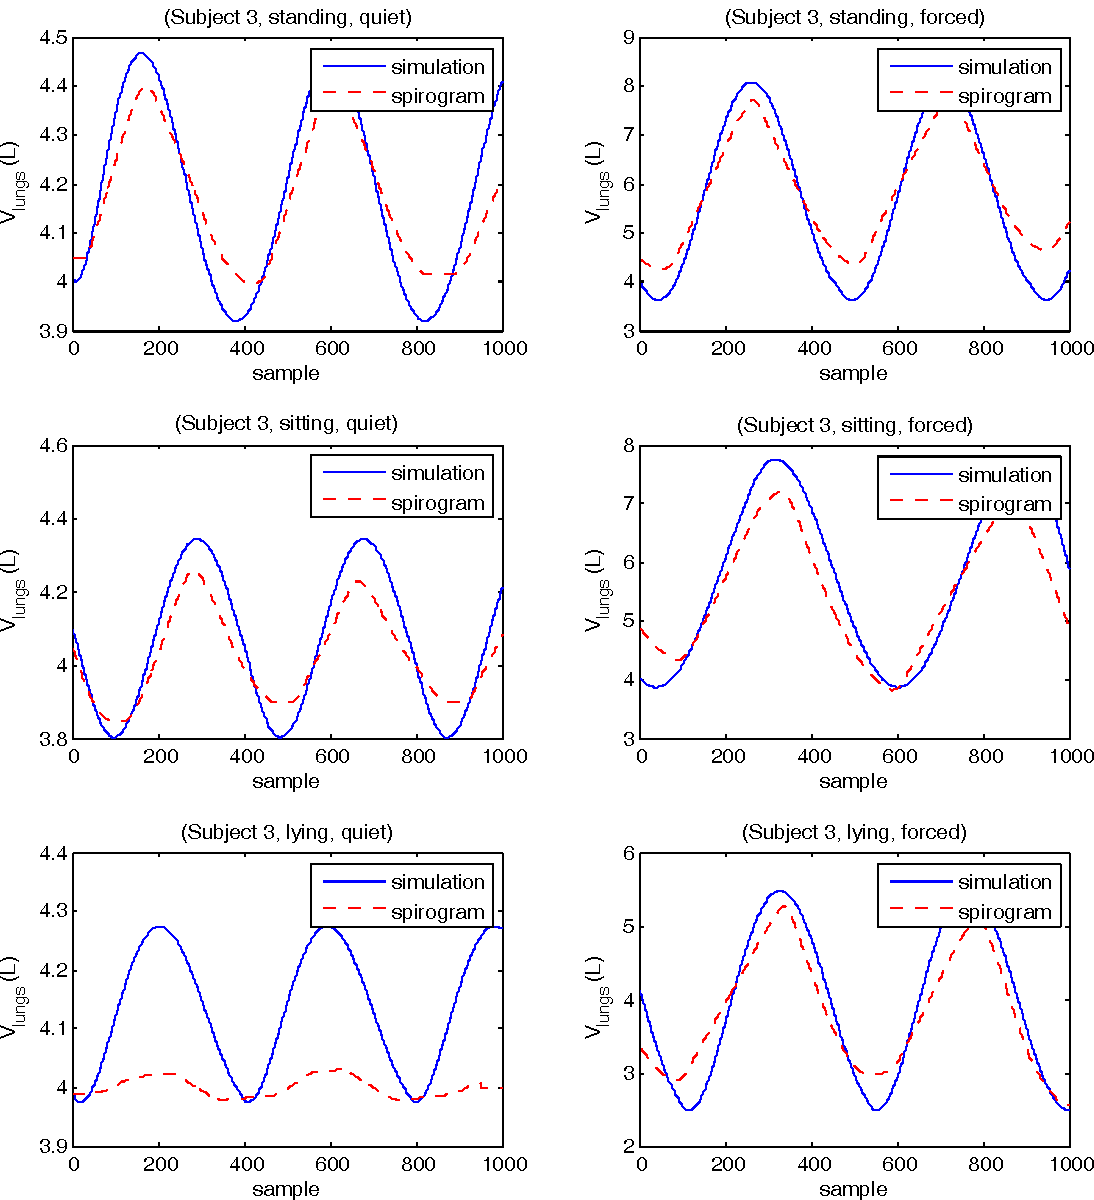
\includegraphics[width=1\textwidth]{pics/to}
	\caption[Simulation and spirometry data from subject 3]{\label{appA:fig:p3}Simulation and spirometry data from subject 3.}
\end{figure}









%%%%%%%%%%%%%%%
%APPENDIX B
%%%%%%%%%%%%%%%
\chapter{\label{appendixB}Bland-Altman Plots for Simulation and Spirometry Data}
\markboth{Appendix B - Bland-Altman Plots for Simulation and Spirometry Data}{}

This section presents the Bland-Altman plots obtained from spirometry and simulation on three subjects. 
A blue dashed-dotted line for zero mean difference along with two red dashed lines at $\pm~1.96~\times~SD_{diff}$ from the mean are included in the plots. 

\newpage
\section{\label{appendixB:p1}Subject 1}

\begin{figure}[H]
	\centering
	 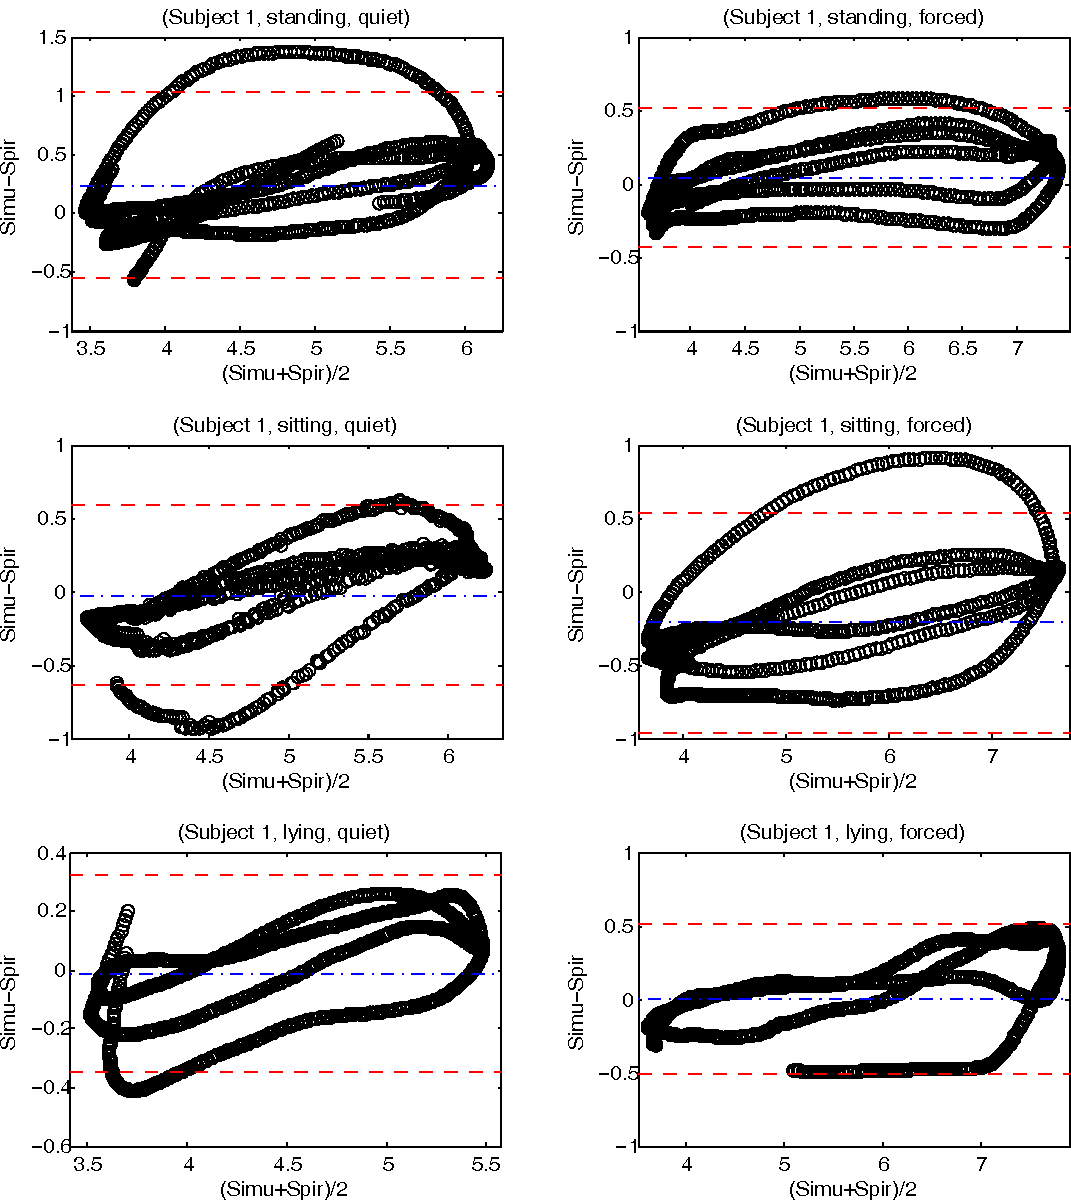
\includegraphics[width=1\textwidth]{pics/ba_p1_det}
	\caption[Bland-Altman plots for simulation and spirometry data from subject 1]{\label{appB:fig:p1}Bland-Altman plots for simulation and spirometry data from subject 1.}
\end{figure}

\newpage
\section{\label{appendixB:p2}Subject 2}

\begin{figure}[H]
	\centering
	 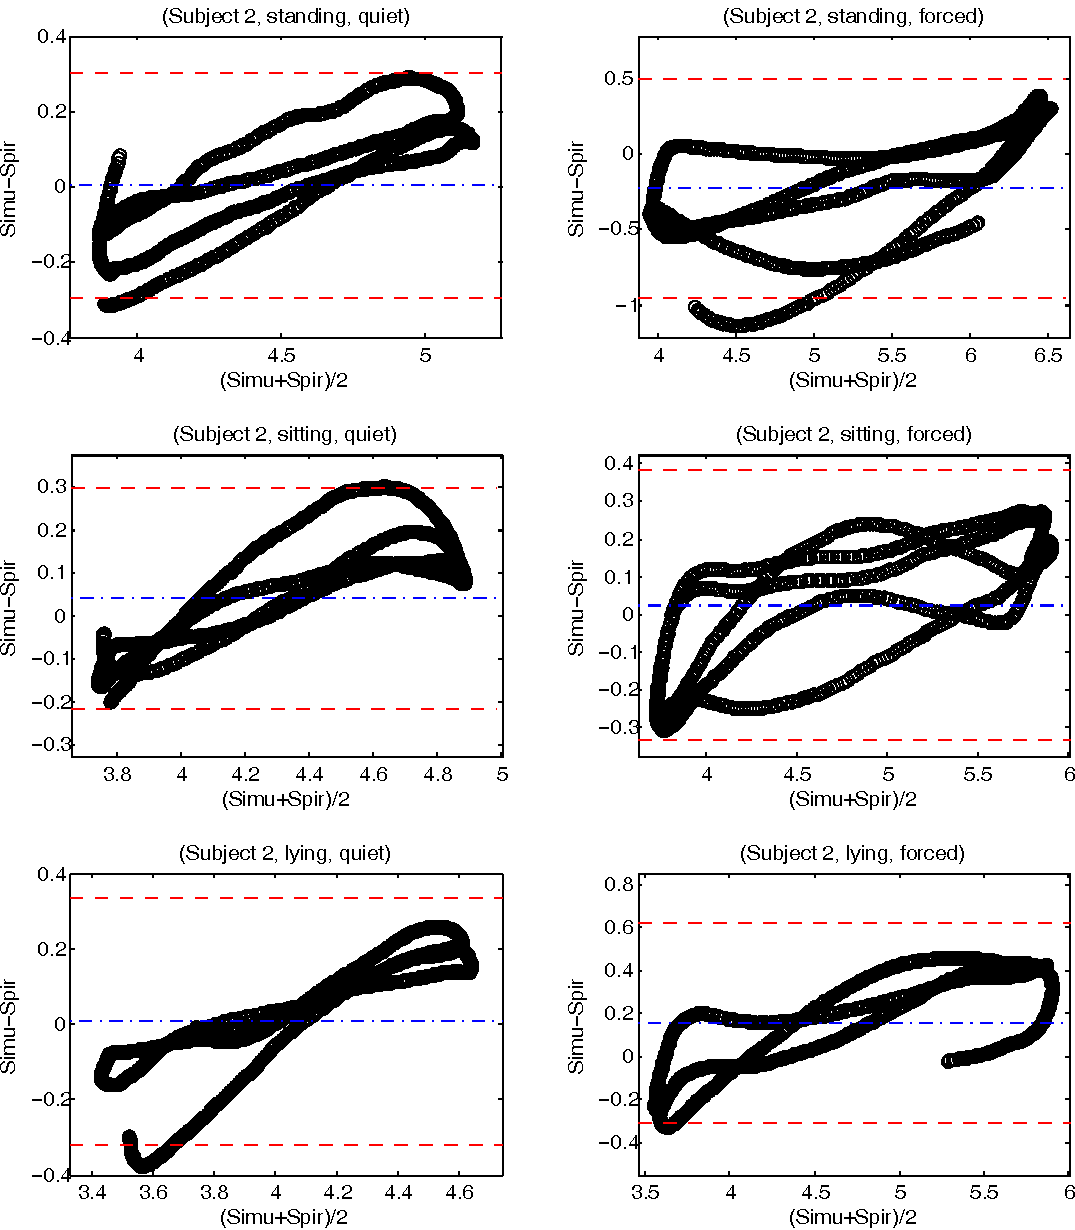
\includegraphics[width=1\textwidth]{pics/ba_p2_det}
	\caption[Bland-Altman plots for simulation and spirometry data from subject 2]{\label{appB:fig:p2}Bland-Altman plots for simulation and spirometry data from subject 2.}
\end{figure}

\newpage
\section{\label{appendixB:p3}Subject 3}

\begin{figure}[H]
	\centering
	 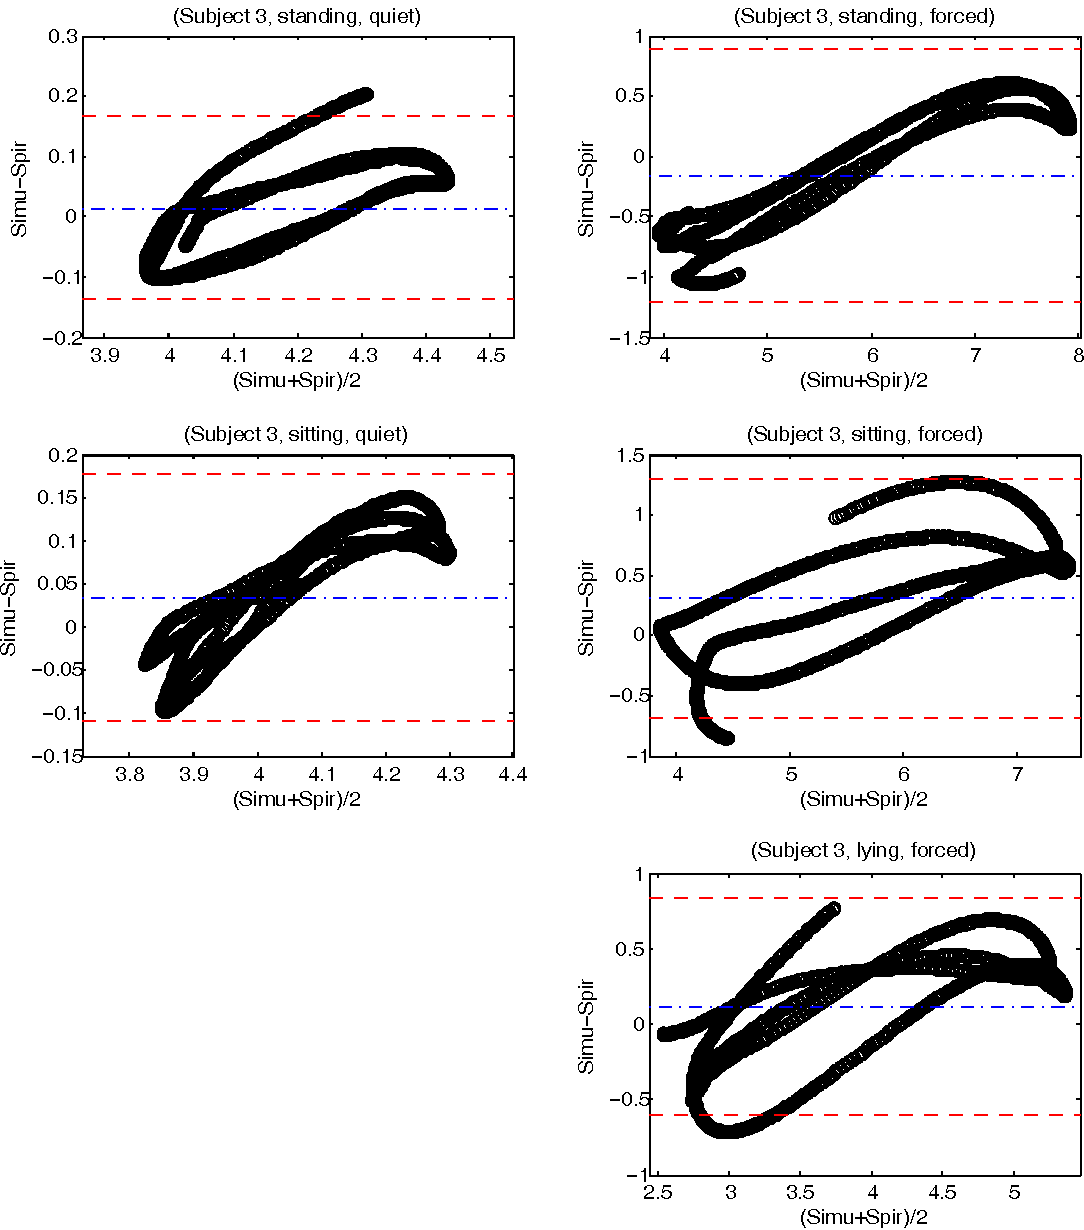
\includegraphics[width=1\textwidth]{pics/ba_p3_det}
	\caption[Bland-Altman plots for simulation and spirometry data from subject 3]{\label{appB:fig:p3}Bland-Altman plots for simulation and spirometry data from subject 3.}
\end{figure}